\maketitle

% =========================================================
% Frontmatter (Titel/Abstract/Danksagung) OHNE Kopfzeile
% =========================================================
\pagestyle{empty} % oder 'empty', wenn du GAR keine Kopf-/Fußzeile willst

\renewcommand{\headrulewidth}{0pt}
\newpage
\clearpage
\hfuzz=12pt       % suppress warnings due to extenstion onto page margins
{
%\fontsize{14pt}{20pt}\textbf{Kurzreferat}\\ \\
\section*{Kurzreferat}
%\fontsize{11pt}{12pt}\textbf{\Autor}
\subsection*{\Autor}
\vspace{0.3cm}
\textbf{Thema der Arbeit}
    \par \begingroup \leftskip=3em %\noindent
\Titel 
    \par \endgroup

\vspace{0.3cm}
\textbf{Stichworte}
    \par \begingroup \leftskip=3em % \noindent
\Stichworte
    \par \endgroup

\vspace{0.3cm}
\textbf{Kurzzusammenfassung}
    \par \begingroup \leftskip=3em % \noindent
\Zusammenfassung
    \par \endgroup


%\vspace{1.0cm}
\subsection*{\Autor}
%\textbf{\Autor}

\vspace{0.3cm}
\textbf{Title of Thesis}
    \par \begingroup \leftskip=3em %\noindent
\TitelEN
    \par \endgroup
    
\vspace{0.3cm}
\textbf{Keywords}
    \par \begingroup \leftskip=3em %\noindent
\StichworteEN
    \par \endgroup
    
\vspace{0.3cm}
\textbf{Abstract}
    \par \begingroup \leftskip=3em %\noindent
\ZusammenfassungEN
    \par \endgroup
}
\clearpage
\thispagestyle{empty}

\section*{Danksagung}
An dieser Stelle möchte ich mich bei allen bedanken, die mich bei der Anfertigung dieser Bachelorarbeit unterstützt haben.

Mein besonderer Dank gilt Herrn Prof. Dr.-Ing. Alexander Frenkel von der HAW Hamburg für die Betreuung dieser Arbeit sowie für die fachlichen Anregungen und konstruktiven Hinweise während der gesamten Bearbeitungszeit.

Ebenso danke ich Herrn Bernd Lüerß für die Unterstützung als industrieller Betreuer sowie als externer Zweitprüfer dieser Arbeit. Die praxisnahe Begleitung und die fachlichen Diskussionen haben wesentlich zum erfolgreichen Abschluss dieser Bachelorarbeit beigetragen.

Darüber hinaus bedanke ich mich bei dem Team der Technologieplattform für die Unterstützung im Rahmen des Gesamtprojekts.

Mein Dank gilt außerdem den Kolleginnen und Kollegen der Abteilung Motion für die Unterstützung bei der Problemlösung sowie der Abteilung Automation für die Mitwirkung bei der Konzeptentwicklung.

Des Weiteren danke ich dem Team der Prototyping Service Production für die Fertigung der benötigten Frästeile.

Abschließend möchte ich mich bei meiner Familie und meinen Freunden bedanken, die mich während meines Studiums und insbesondere während der Bearbeitung dieser Arbeit stets unterstützt und motiviert haben.
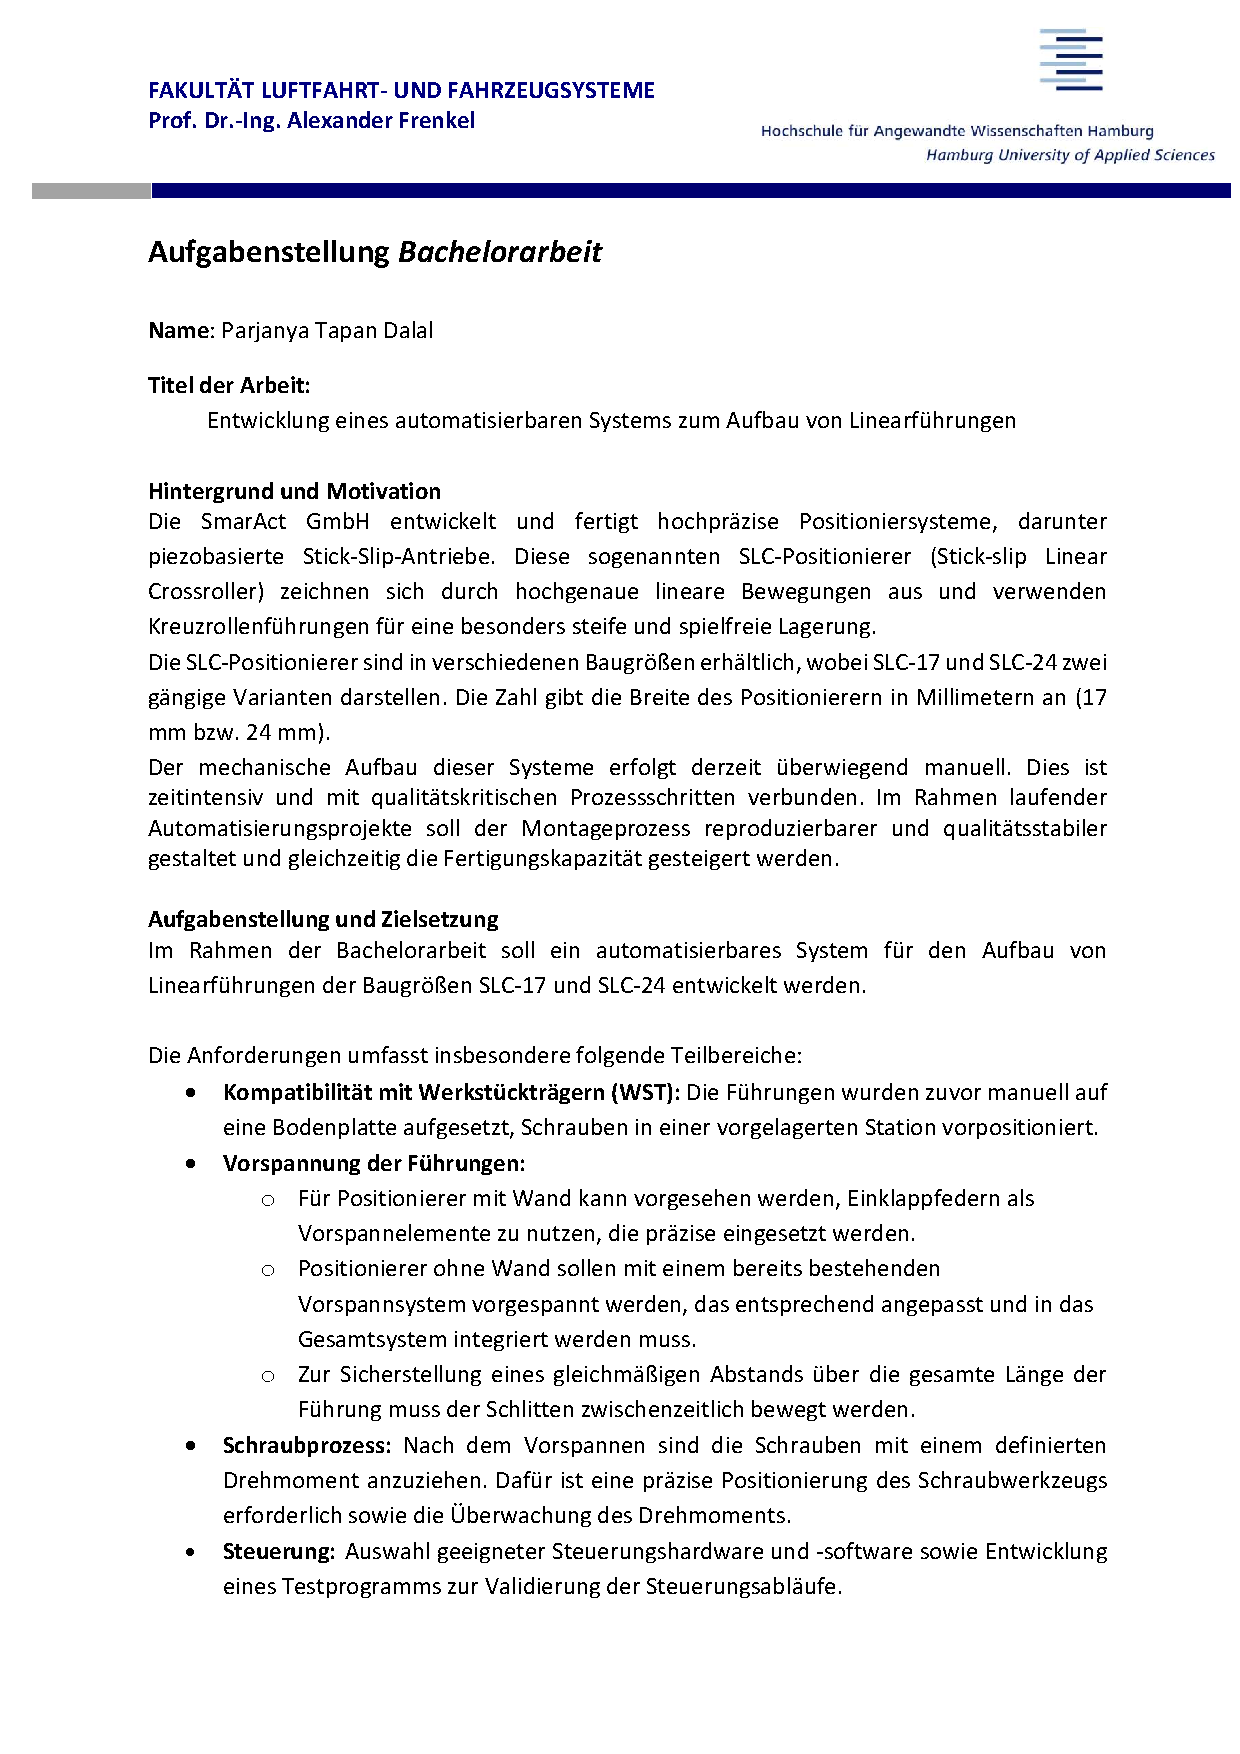
\includepdf[pages={-}]{misc/Background/aufgabenstellung.pdf}

\clearpage

% =========================================================
% Frontmatter-Nummerierung (römisch)
% =========================================================
\pagenumbering{Roman}
\setcounter{page}{1}

% =========================================================
% AB HIER: Kopfzeile AKTIV (ab Inhaltsverzeichnis)
% =========================================================
\pagestyle{fancy}

% Sicherheit: genügend Platz für Header
\setlength{\headheight}{18pt}

% Sicherheit: Kopfzeilenlinie erzwingen (falls irgendwo auf 0 gesetzt)
\renewcommand{\headrulewidth}{0.4pt}
\renewcommand{\footrulewidth}{0pt}

% Inhaltsverzeichnis
\maintoc
\clearpage

% Abbildungs- und Tabellenverzeichnis
\listoffigures
\clearpage
\listoftables
\clearpage

% Abkürzungsverzeichnis
\printglossary[type=acronym,style=acrotab, title = Abkürzungen]
% Symbolverzeichnis
\printglossary[type=symbols, style=symboltablr, title = Nomenklatur]
\clearpage

% =========================================================
% Ab hier: Hauptteil (arabisch)
% =========================================================
\setcounter{table}{0}
\renewcommand{\arraystretch}{1.15}
\pagenumbering{arabic}
